\PassOptionsToPackage{unicode=true}{hyperref} % options for packages loaded elsewhere
\PassOptionsToPackage{hyphens}{url}
%

\documentclass[12pt,AutoFakeBold,AutoFakeSlant]{article}
% 12pt == 小四

\usepackage{amssymb,amsmath}
\usepackage{ifxetex,ifluatex}
\usepackage{unicode-math}

% use upquote if available, for straight quotes in verbatim environments
\IfFileExists{upquote.sty}{\usepackage{upquote}}{}
% use microtype if available

\IfFileExists{microtype.sty}{%
\usepackage[]{microtype}
\UseMicrotypeSet[protrusion]{basicmath} % disable protrusion for tt fonts
}{}

\usepackage{hyperref}
\hypersetup{
            pdfborder={0 0 0},
            breaklinks=true}
\urlstyle{same}  % don't use monospace font for urls

\usepackage{longtable,booktabs}

% Fix footnotes in tables (requires footnote package)
\IfFileExists{footnote.sty}{\usepackage{footnote}\makesavenoteenv{longtable}}{}
\setlength{\emergencystretch}{3em}  % prevent overfull lines
\providecommand{\tightlist}{%
  \setlength{\itemsep}{0pt}\setlength{\parskip}{0pt}}

\usepackage{fontspec}
\usepackage{ctex}

\usepackage{indentfirst}
\usepackage{fullpage}

\setmainfont{Times New Roman}
\setmonofont{Courier New}
\setCJKmainfont{SimSun}
\setCJKmonofont{SimSun}

\newcommand{\ms}[1]{\texttt{#1}}

\usepackage{listings}
\lstset{basicstyle=\ttfamily,breaklines=true}

\usepackage[table,svgnames]{xcolor}
\usepackage{cellspace}
\usepackage{etoolbox}
\definecolor{headercolor}{RGB}{198,217,241} % #c6d9f1

\linespread{1.5} % https://tex.stackexchange.com/questions/30073/why-is-the-linespread-factor-as-it-is
\usepackage[tmargin=1in,bmargin=1in,lmargin=1.25in,rmargin=1.25in]{geometry} % word-like, see https://tex.stackexchange.com/questions/35892/latex-optimal-settings-for-ms-word-like-document
\setlength{\arrayrulewidth}{0.5pt}

\AtBeginEnvironment{longtable}{\rowcolors{0}{\ifnumless{\rownum}{3}{white}{headercolor}}{}}
\AtBeginEnvironment{longtable}{\zihao{5}}

\usepackage{nameref}
\makeatletter
\newcommand*{\currentname}{\@currentlabelname}
\makeatother
\newcounter{tablecaption}
\AtBeginEnvironment{longtable}{\stepcounter{tablecaption}\flushright{{\setlength\parskip{0pt}\heiti{表 \arabic{tablecaption} \currentname{}}}}\vspace*{-7pt}} % NOTE: hack since \caption in longtable breaks the current way of setting colors for table header

\newcommand{\headingcellfirst}[1]{\multicolumn{1}{|c|}{\heiti{#1}}} % NOTE: \DeclareRobustCommand has issues
\newcommand{\headingcellmiddle}[1]{\multicolumn{1}{c|}{\heiti{#1}}}
\newcommand{\headingcelllast}[1]{\multicolumn{1}{c|}{\heiti{#1}}}

\usepackage{makecell}
\usepackage{multirow}

\usepackage{mips}

\usepackage{pgf}
\usepackage{tikz}
\usetikzlibrary[arrows,automata]

\usepackage{graphicx}

\begin{document}

{
\setlength{\parskip}{\baselineskip}%

\begin{center}
\zihao{3}
\heiti{计算机组成原理实验报告\\P7 计时器说明文档}
\end{center}
}

\tableofcontents
\newpage

\section{简介}

本文档是 P7 课下“沟通外部设备与计时器”一节的要求,包括计时器的状态转移图及其使用说明。

\section{状态转移图}

以下是两种模式的状态转移图。

圆圈代表状态或操作,圆圈里的文字表示状态;箭头上方(或左方)的文字代表转换条件,下方(或右方)的文字代表状态转换时的附加操作。

\subsection{定时中断模式}

以下是 \ms{mode == 2'b00},也就是定时产生中断时的状态转移图。

\begin{center}
 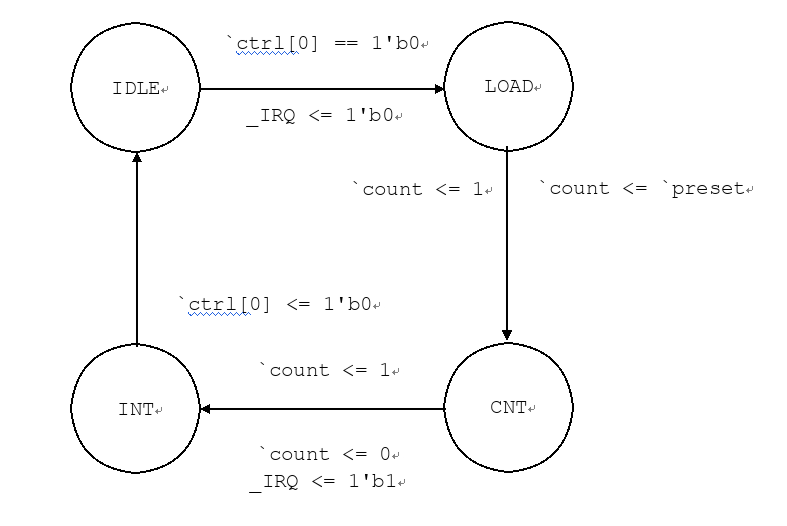
\includegraphics[width=0.7\textwidth]{pipelined3-timer-1.png}
 % pipelined3-timer-1.png: 787x526 px, 140dpi, 14.28x9.54 cm, bb=0 0 405 271
\end{center}

\subsection{连续中断模式}

以下是 \ms{mode != 2'b00},也就是连续产生中断时的状态转移图。

\begin{center}
 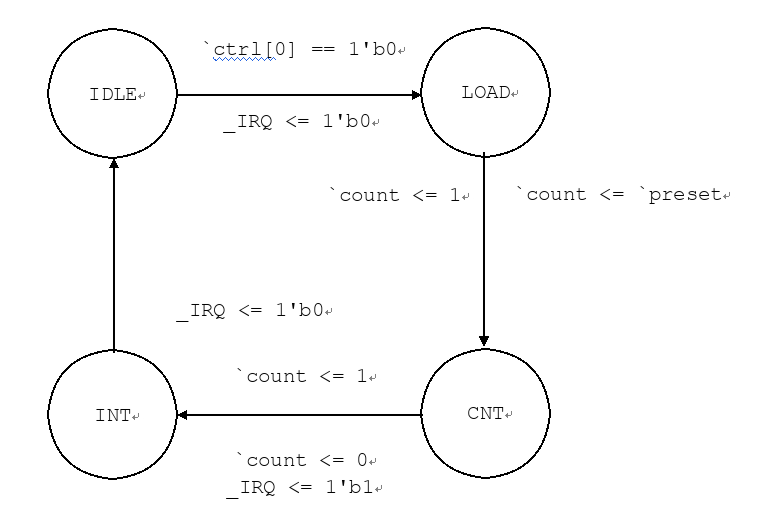
\includegraphics[width=0.7\textwidth]{pipelined3-timer-2.png}
\end{center}

\section{使用说明}

\subsection{基本要求}

无论计时器在什么模式和什么状态下,都有以下的基本要求要遵守。

\begin{enumerate}
\tightlist
\item
\ms{TC} 的内部寄存器只能用读写整个位的模式。
\item
\ms{TC} 的 \ms{count} 寄存器不能被写入。
\item
\ms{TC} 先处理对其内部寄存器的写入请求,无论是否有效。若无写入请求,则进行状态转移。
\end{enumerate}

\subsection{读取操作规范}

读取操作是通过组合逻辑实现的。\ms{TC} 中对内部寄存器的读取,不考虑其状态,只考虑操作地址 \ms{Addr}。各种操作及其对应结果如下表。

\begin{longtable}[]{@{}|l|l|l|l|@{}}
\hline
\headingcellfirst{\ms{Addr}} & \headingcellmiddle{是否可行} & \headingcellmiddle{结果} & \headingcelllast{不可行原因} \\\hline
\endhead\hiderowcolors
\ms{2'b00\~{}2'b01} & 是 & 读出对应的内部寄存器 & --- \\\hline
\ms{2'b11} & 否 & 读出 \ms{32'hXXXXXXXX} & 寄存器数组 \ms{mem} 只定义了 \ms{[0:2]} \\\hline
\end{longtable}

\subsection{写入操作规范}

写入逻辑在真正向对应的寄存器写入值以前,首先对 \ms{Addr} 进行了判断。如果 \ms{Addr == 2'b0},那么就是要写入 \ms{ctrl} 寄存器,写入的高 28 位被忽略。之后不再说明,会直接像整个字被写入那样来描述,但实际上写入情况是有差别的。

由于写入逻辑在同一个时钟周期内优先级较高,所以之后描述的结果,一般都是从写入逻辑所在时钟周期的下一个时钟周期开始描述。

\subsubsection{\ms{IDLE} 状态}

\ms{IDLE} 状态会根据 \ms{`ctrl[0]} 是否使能,来确定是否进入 \ms{LOAD} 状态,并把中断信号设为未激活。

无论处于哪种模式,该状态下,写入 \ms{ctrl} 和 \ms{preset} 都可行。

写入 \ms{ctrl} 会改变对应控制信号的值,写入后立即生效。

若写入了 \ms{`ctrl[0]},则会改变 \ms{TC} 的使能。

若写入了 \ms{`ctrl[2:1]},则会改变当前模式。

写入的 \ms{`ctrl[3]} 会影响中断使能。

写入 \ms{preset} 会影响预置数的值。

写入 \ms{count} 不可行,但是不会产生影响,因为 \ms{count} 会在进入 \ms{LOAD} 状态时被覆盖。

\subsubsection{\ms{LOAD} 状态}

\ms{LOAD} 状态会从 \ms{preset} 里取数,并写入 \ms{count} 里,然后进入 \ms{CNT} 状态。

无论处于哪种模式,该状态下,写入 \ms{ctrl} 和 \ms{preset} 都可行。

写入 \ms{ctrl} 会改变对应控制信号的值,写入后虽然控制信号的改变会立即生效,但是除了 \ms{`ctrl[3]} 不会立即发挥作用。

若写入了 \ms{`ctrl[0]},则会在进入 \ms{CNT} 状态后马上回到 \ms{IDLE} 状态。

若写入了 \ms{`ctrl[2:1]},则会改变当前模式。

写入的 \ms{`ctrl[3]} 会影响中断使能。

写入 \ms{preset} 会影响预置数的值。

写入 \ms{count} 不可行,但是不会产生影响,因为 \ms{count} 会在该状态被覆盖。

\subsubsection{\ms{CNT} 状态}

\ms{CNT} 状态会在每次计数时判断 \ms{enable} 的值。若 \ms{enable == 1'b0},则进入 \ms{IDLE} 状态。否则若 \ms{count > 1},\ms{count} 自减一。否则,令 \ms{count = 0, irq = 1'b1},进入 \ms{INT} 状态。

无论处于哪种模式,该状态下,写入 \ms{ctrl} 和 \ms{preset} 都可行。

写入 \ms{ctrl} 会改变对应控制信号的值,控制信号的改变会立即生效。

若写入的 \ms{`ctrl[0] == 1'b0},则会进入 \ms{IDLE} 状态。

若写入了 \ms{`ctrl[2:1]},则会改变当前模式。

写入的 \ms{`ctrl[3]} 会影响中断使能。

写入 \ms{preset} 不会立即影响预置数的值,会在下次进入 \ms{LOAD} 状态后影响。

写入 \ms{count} 不可行,但是会产生影响。若写入的 \ms{count == 32'b0 || count == 32'b1},那么 \ms{count} 会再变为 0,然后进入 \ms{INT} 状态。若写入的 \ms{count >= 32'b2},那么 \ms{count} 寄存器的值会直接改变,继续往下计数。

\subsubsection{\ms{INT} 状态}

该状态下会根据模式判断禁用使能(若 \ms{`ctrl[2:1] == 2'b00})或禁用中断(其它情况)。然后,进入 \ms{IDLE} 状态。

无论处于哪种模式,该状态下,写入 \ms{ctrl} 和 \ms{preset} 都可行。写入 \ms{ctrl} 会改变对应控制信号的值,控制信号的改变会立即生效。

若写入的 \ms{`ctrl[0] == 1'b0},则无论模式,下次进入 \ms{IDLE} 状态后,一定不会自动重新进入 \ms{LOAD} 状态。若写入的 \ms{`ctrl[0] == 1'b1},则实际上无效。

若写入了 \ms{`ctrl[2:1]},则会改变当前模式。

写入的 \ms{`ctrl[3]} 会影响中断使能。

写入 \ms{preset} 不会立即影响预置数的值,会在下次进入 \ms{LOAD} 状态后影响。

写入 \ms{count} 不可行,但是不会产生影响,因为下次进入 \ms{LOAD} 状态时,\ms{count} 的值会被覆盖。

\section{注释}

本文档使用的与计时器相关的名称,如状态名称、内部寄存器名称等,均以课上提供的 \ms{P7\_standard\_TC\_2019.v} 为准,和 CPU 主设计文档中的 \ms{TC} 对应部分不一样。差异主要在命名惯例方面,因为 CPU 主设计文档中的 \ms{TC} 功能,与课上提供的没有差异,只是它的修改版。

课上提供的 \ms{P7\_standard\_TC\_2019.v} 永久链接:\url{http://cscore.net.cn/assets/courseware/v1/71af5d8b232b93d8de77c1b3026f3158/asset-v1:Internal+B3I062410+2019_T1+type@asset+block/P7_standard_TC_2019.v}

\end{document}

